\section{Genetic Heterogeneity in Multi-Agent Systems}

\begin{frame}{Defining Heterogeneity}

\Large

heterogeneity: NOT absolute homogeneity
\begin{itemize}
\item all agents \textit{completely} identical
\item intuition: standing between two mirrors
\end{itemize}

\vspace{2ex}

necessary to solve leader election problem \cite{angluin1980local,banda2015configuration}

\end{frame}

\begin{frame}{Multiple Sources of Heterogeneity}

heterogeneous groups can solve leader election:
\begin{itemize}
\item configuration \cite{frederickson1987electing}
\item state \cite{banda2015configuration}
\item connectivity \cite{antonoiu1996self}
\item stochasticity \cite{itai1981symmetry}
\end{itemize}

\vspace{2ex}

at least \textit{some} heterogeneity seems essential
\begin{itemize}
\item ... and is ubiquitous in multi-agent systems \cite{atodd2015quantitative, perna2012individual, fayeez2017h}
\end{itemize}


\end{frame}

\begin{frame}{Genetic Heterogeneity}

\Large

\begin{itemize}
\item configuration heterogeneity
\item specialization
\begin{itemize}
\item division of labor \cite{potter2001heterogeneity}
\item different capabilities (e.g., ground and aerial robots) \cite{gomes2015cooperative, mathews2012supervised}
\item variation in unit-to-unit hardware \cite{pugh2007parallel, duarte2016evolution}
\end{itemize}
\end{itemize}

alternative: plasticity \cite{tuci2008evolving}

\end{frame}

\begin{frame}{Credit Assignment Problem}

\Large

evolutionary approach: need metric of genome performance for selection
\begin{itemize}
\item clonal groups: exploit symmetry, just use group performance metric
\item non-clonal groups: ???
\end{itemize}

\textbf{crux:} nailing down value of individual contributions to group performance is nontrivial \cite{panait2005cooperative}

\end{frame}

\begin{frame}{Credit Assignment Problem}

\Large

\begin{itemize}
\item weakening selection \cite{knudson2010coevolution, waibel2009genetic}
\item incentivizing defection \cite{knudson2010coevolution, waibel2009genetic}
\item context dependence \cite{gomes2015cooperative}
\end{itemize}

\pause

intuition: hypothetical hockey examples

\end{frame}

\begin{frame}{Credit Assignment Problem: Weakening Selection}

\begin{columns}
\begin{column}{0.5\textwidth}
{\Large
randomly drawn teams of professional and amateur players
\begin{align*}
\bm{\downarrow}
\end{align*}
own performance weakly correlates with team performance

}
\end{column}
\begin{column}{0.5\textwidth}


\begin{figure}
\begin{subfigure}[b]{\textwidth}
\begin{columns}
\begin{column}{0.05\textwidth}
\caption{}
\label{fig:professional-hockey}
\end{column}
\begin{column}{0.95\textwidth}
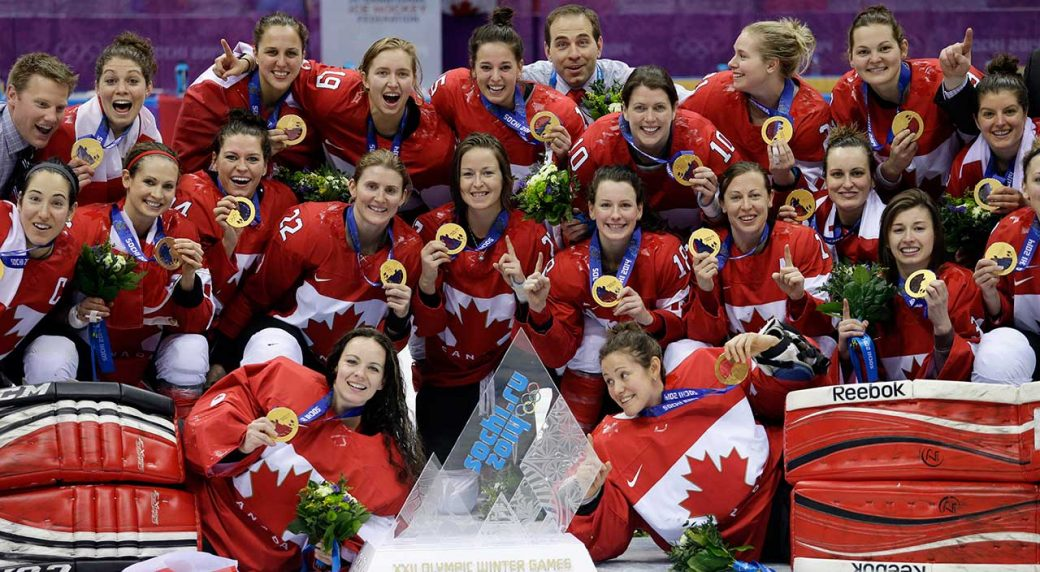
\includegraphics[width=\textwidth]{professional-hockey}
\end{column}
\end{columns}
\end{subfigure}%

\begin{subfigure}[b]{\textwidth}
\begin{columns}
\begin{column}{0.05\textwidth}
\caption{}
\label{fig:amateur-hockey}
\end{column}
\begin{column}{0.95\textwidth}
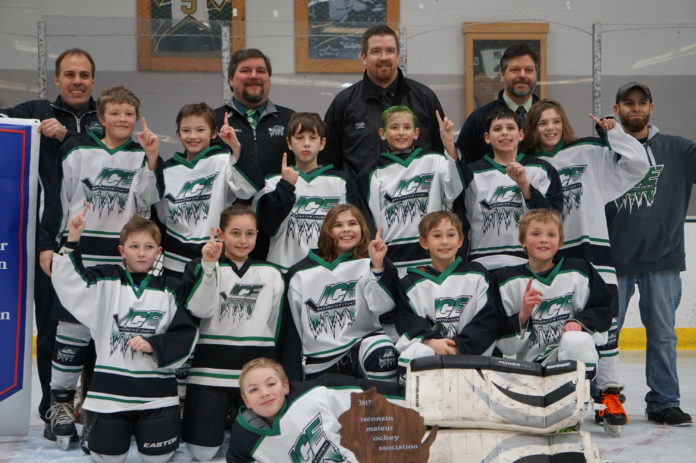
\includegraphics[width=\textwidth]{amateur-hockey}
\end{column}
\end{columns}
\end{subfigure}

\caption{
Professional (\ref{fig:professional-hockey}) and amateur (\ref{fig:amateur-hockey}) hockey players.
}

\end{figure}
\end{column}
\end{columns}

\end{frame}

\begin{frame}{Credit Assignment Problem: Weakening Selection}

\vspace{2ex}

{\Large
selection gets weaker as groups get bigger
}

\begin{figure}
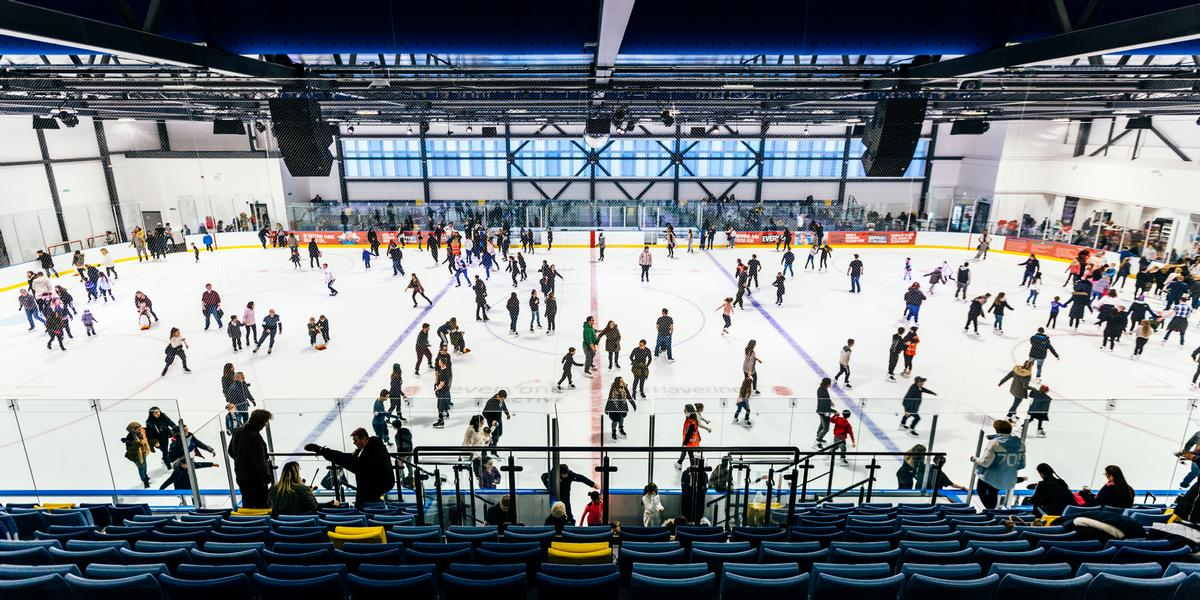
\includegraphics[width=\textwidth]{crowded-rink}
\caption{A crowded hockey rink.}
\label{fig:crowded-rink}
\end{figure}


\end{frame}

\begin{frame}{Credit Assignment Problem: Incentivizing Defection}

\begin{columns}
\begin{column}{0.5\textwidth}
{\Large
players rewarded for goals \textit{they} score
\begin{align*}
\bm{\downarrow}
\end{align*}
players take ``Slap Shots'' instead of passing
\begin{align*}
\bm{\downarrow}
\end{align*}
overall, team makes fewer goals
}
\end{column}
\begin{column}{0.5\textwidth}
\begin{figure}
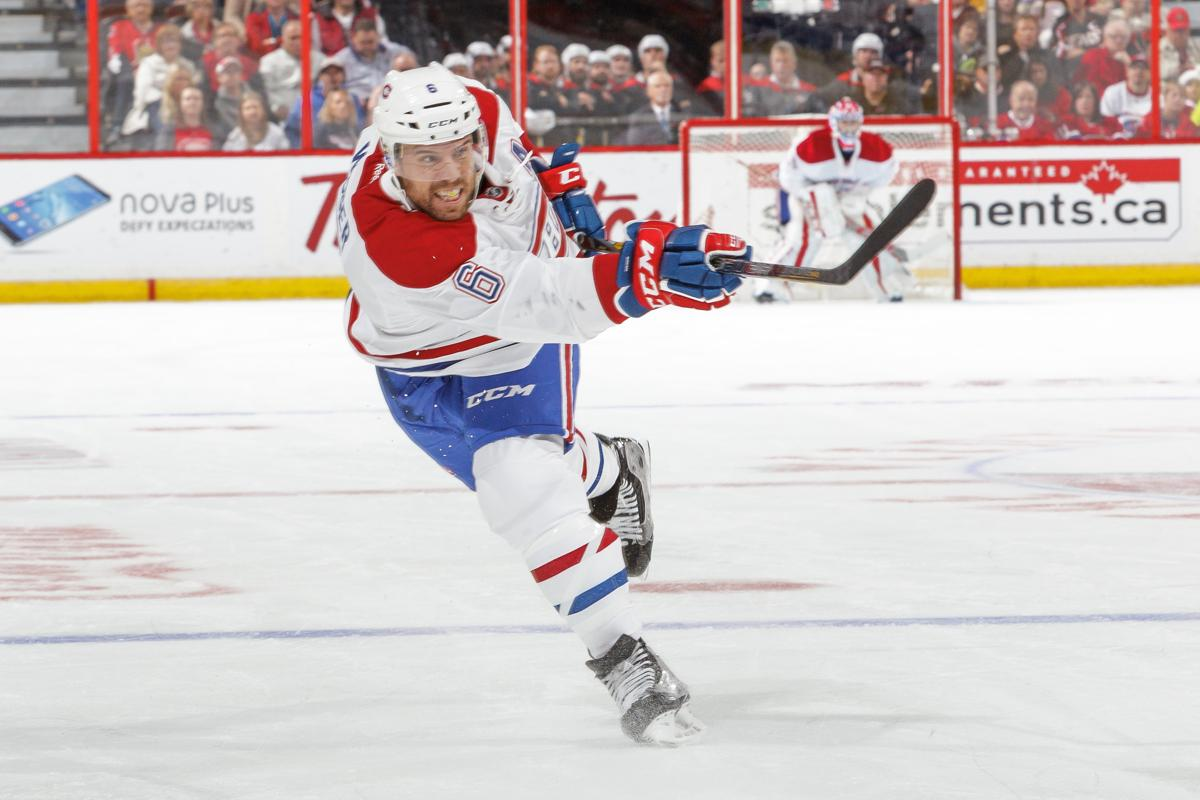
\includegraphics[width=\textwidth]{slap-shot}
\caption{
A ``Slap Shot.''
}
\label{fig:slap-shot}
\end{figure}
\end{column}
\end{columns}

\end{frame}

\begin{frame}{Credit Assignment Problem: Context Dependence}

\begin{columns}
\begin{column}{0.5\textwidth}
\Large
success of Royal Road passer depends on partner near the goal
\end{column}
\begin{column}{0.5\textwidth}
\begin{figure}
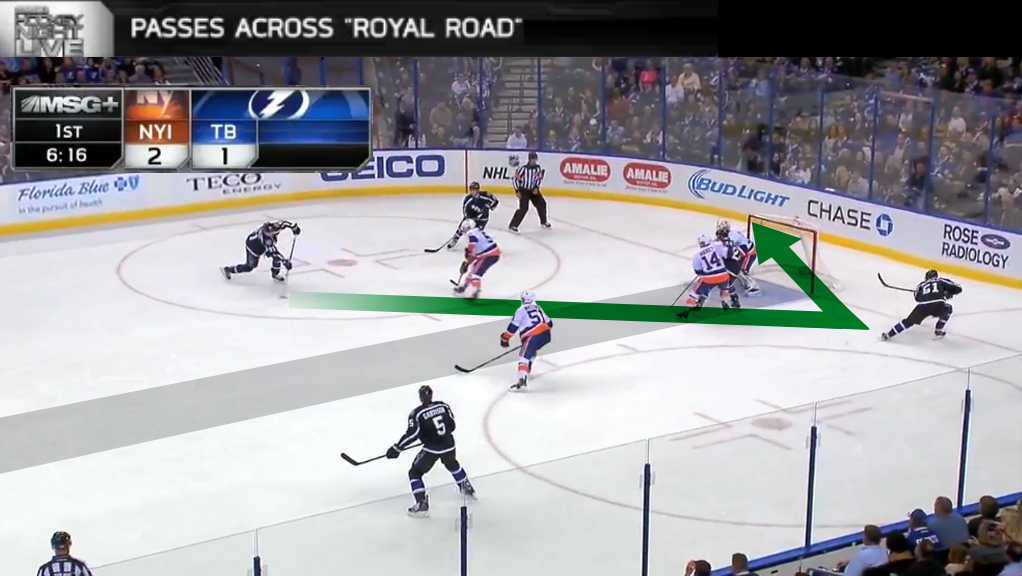
\includegraphics[width=\textwidth]{royal-road-pass}
\caption{
A pass across the ``Royal Road.''
}
\label{fig:royal-road-pass}
\end{figure}
\end{column}
\end{columns}


\end{frame}


\begin{frame}{Credit Assignment Problem}

three approaches:
\begin{itemize}
\item calculating fitness as the difference between group performance and estimated group performance without the contributions of an agent \cite{knudson2010coevolution}
\item designing individual payoffs in order to align with individual contribution to group success \cite{waibel2009genetic}
\item cooperative co-evolution, where individuals in distinct subpopulations corresponding to distinct roles are selected by evaluation only with the best-performing individuals from other subpopulations \cite{gomes2015cooperative}
\end{itemize}

\end{frame}
